\documentclass[tikz,border=9pt]{standalone}
\usepackage{amsmath,amssymb}
\usetikzlibrary{arrows.meta,positioning,calc}
\begin{document}
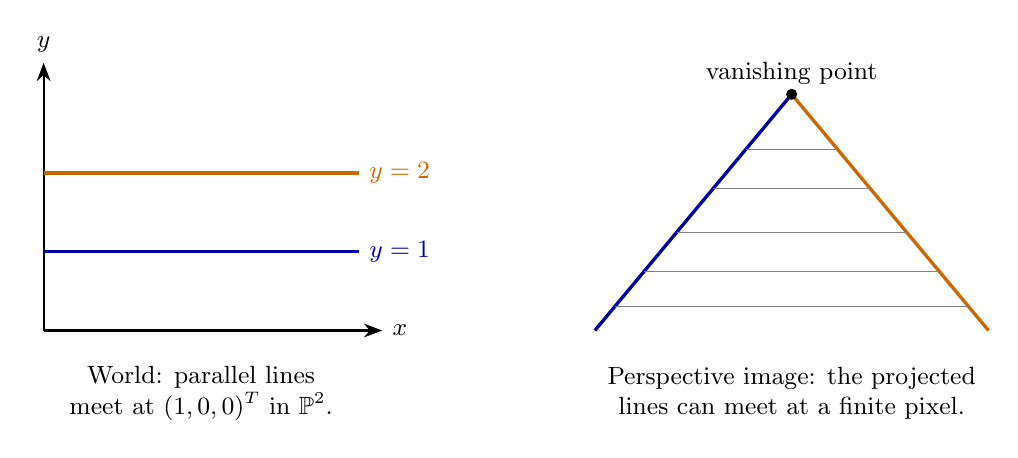
\begin{tikzpicture}[font=\small,arr/.style={-{Stealth},thick},box/.style={draw=blue!55!black,rounded corners,fill=blue!4,align=center,text width=2.9cm,minimum height=1.05cm}]

\draw[arr] (0,0)--(4.3,0) node[right]{$x$};\draw[arr] (0,0)--(0,3.4) node[above]{$y$};
\draw[very thick,blue!65!black] (0,1)--(4,1) node[right]{$y=1$};
\draw[very thick,orange!80!black] (0,2)--(4,2) node[right]{$y=2$};
\node[align=center] at (2,-.8){World: parallel lines\\meet at $(1,0,0)^T$ in $\mathbb P^2$.};
\begin{scope}[shift={(7,0)}]
\coordinate (v) at (2.5,3);\draw[very thick,blue!65!black] (0,0)--(v);
\draw[very thick,orange!80!black] (5,0)--(v);
\foreach \y in {.3,.75,1.25,1.8,2.3} {\draw[gray] ({\y/3*2.5},\y)--({5-\y/3*2.5},\y);}
\fill (v) circle(2pt) node[above]{vanishing point};
\node[align=center] at (2.5,-.8){Perspective image: the projected\\lines can meet at a finite pixel.};
\end{scope}

\end{tikzpicture}
\end{document}
